
\medskip

Le diagramme ci-dessous représente, pour six pays, la quantité de nourriture gaspillée (en kg) par habitant en 2010.

\begin{center}
	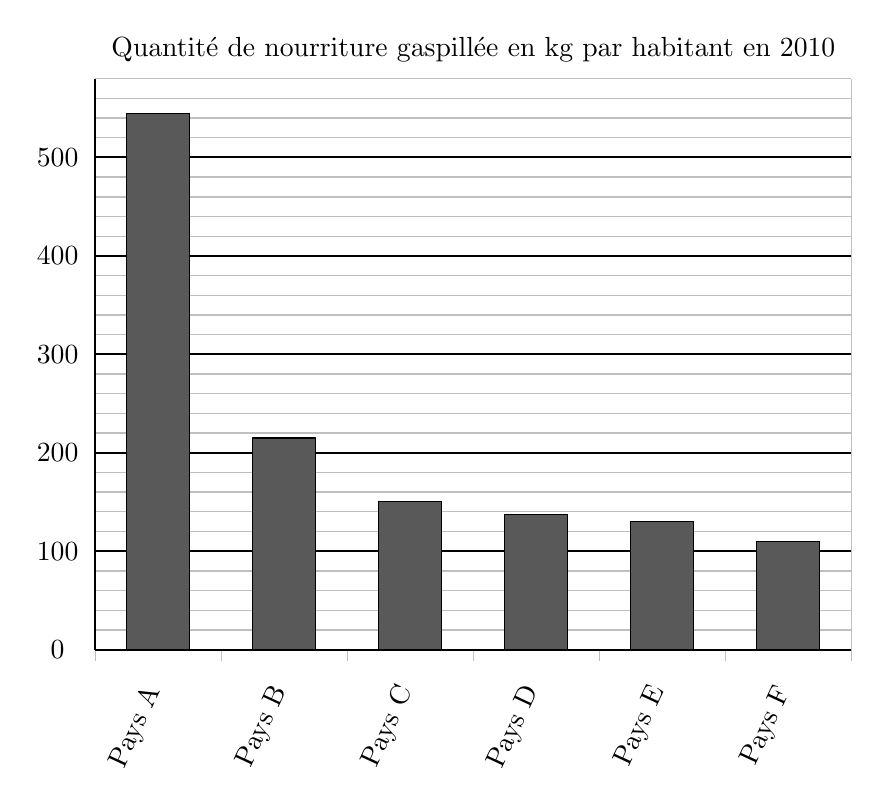
\begin{tikzpicture}[y=0.125mm,x=4mm]% l'échelle ridicule proposée ici est celle du sujet original
		\draw [xstep=24,ystep=20,gray!50,line width=0.5pt] (0,0) grid (24,580);
		\foreach \a in {0,4,...,24}{
		\draw[gray!50,line width=0.5pt] (\a,0)--(\a,-4pt);}	
		\draw [xstep=24.1,ystep=100,black,line width=0.7pt] (0,0) grid (24,580);	
		\foreach \o in {0,100,...,500}{
			\node at (-1.2,\o) {\o};}
		
		\draw[fill=black!65] ( 1,0) rectangle (3 ,545);	
		\node[rotate=65,left] at(2,-30) {Pays A};
		\draw[fill=black!65] ( 5,0) rectangle (7 ,215);
		\node[rotate=65,left] at(6,-30) {Pays B};
		\draw[fill=black!65] ( 9,0) rectangle (11,150);	
		\node[rotate=65,left] at(10,-30) {Pays C};
		\draw[fill=black!65] (13,0) rectangle (15,137.5);
		\node[rotate=65,left] at(14,-30) {Pays D};
		\draw[fill=black!65] (17,0) rectangle (19,130);	
		\node[rotate=65,left] at(18,-30) {Pays E};
		\draw[fill=black!65] (21,0) rectangle (23,110);
		\node[rotate=65,left] at(22,-30) {Pays F};
		\node at (12,610){Quantité de nourriture gaspillée en kg par habitant en 2010};
	\end{tikzpicture}
\end{center}

\begin{enumerate}
	\item Donner approximativement la quantité de nourriture gaspillée par un habitant du pays D en 2010.	
	\item Peut-on affirmer que le gaspillage de nourriture d'un habitant du pays F représente environ un cinquième du gaspillage de nourriture d'un habitant du pays A ?	
	\item On veut rendre compte de la quantité de nourriture gaspillée pour d'autres pays. On réalise alors le tableau ci-dessous à l'aide d'un tableur. \hfill \textit{Rappel :} 1 tonne = \np[kg]{1000}.	

\medskip

	\begin{tabularx}{\linewidth}{|>{\columncolor[gray]{.8} \rule[-2.5mm]{0mm}{7mm} \centering \arraybackslash \sffamily} m{5mm}| >{\centering \arraybackslash} p{1.5cm} | *{3}{>{\centering \arraybackslash\rule[-2.5mm]{0mm}{7mm}}X|}} \hline
	\rowcolor[gray]{.8}	&\textsf{A}&\textsf{B}&\textsf{C}&\textsf{D}\\ \hline
		1& &\parbox{\linewidth}{
			\rule{0pt}{10pt}Quantité de nourriture gaspillée par habitant en 2010 (en kg)\rule[-4pt]{0pt}{1pt}}
		&\parbox{\linewidth}{Nombre d'habitants en 2010 (en millions)} 
		&\parbox{\linewidth}{Quantité totale de nourriture gaspillée (en tonnes)}\\ \hline	
	2 & Pays X & 345 & 10,9 & \np{3760500}\\ \hline	
	3 & Pays Y & 212 & 9,4  &             \\ \hline
	4 & Pays Z & 135 & 46,6 &             \\ \hline
	\end{tabularx}

	\begin{enumerate}
		\item  Quelle est la quantité totale de nourriture gaspillée par les habitants du pays X en 2010 ?		
		\item Voici trois propositions de formule, recopier sur votre copie celle qu'on a saisie dans
		la cellule \textsf{D2} avant de l'étirer jusqu'en \textsf{D4}.
		
		\renewcommand{\arraystretch}{1.5}
		\begin{tabularx}{\linewidth}{|*{3}{>{\centering \arraybackslash} X|}} \hline
			\textbf{Proposition 1}&\textbf{Proposition 2}&\textbf{Proposition 3}\\ \hline
			\textsf{=B2*C2*\np{1000000}}&\textsf{=B2*C2}& \textsf{=B2*C2*\np{1000}}\\ \hline
		\end{tabularx}
	\end{enumerate}
\end{enumerate}

\vspace{0,5cm}

